\documentclass[10pt, physics]{homework}

\usepackage{hyperref}
\usepackage{graphicx}

\author{Jackson Petty}
\title{Assignment 2}
\course{PHYS 356}
\due{21 February 2018}

\begin{document}
	\begin{problem}
		Test the central limit theorem by creating plots similar to the figures shown in the Wikipedia page for ``central limit theorem''. 
		\begin{parts}
			\part[part:1:a] Show the distribution of mean values of $N$ random variables obtained from a uniform distribution for increasing numbers of $N$ (i.e., $N = 2, 5, 20, 200)$ and compare each distribution with a Gaussian with the same mean and variance as the obtained distribution.
			\part[part:1:b] Do the same as ~\ref{part:1:a} but using the distribution in problem 4 of problem set 1, with $a = 2$.
		\end{parts}
	\end{problem}
	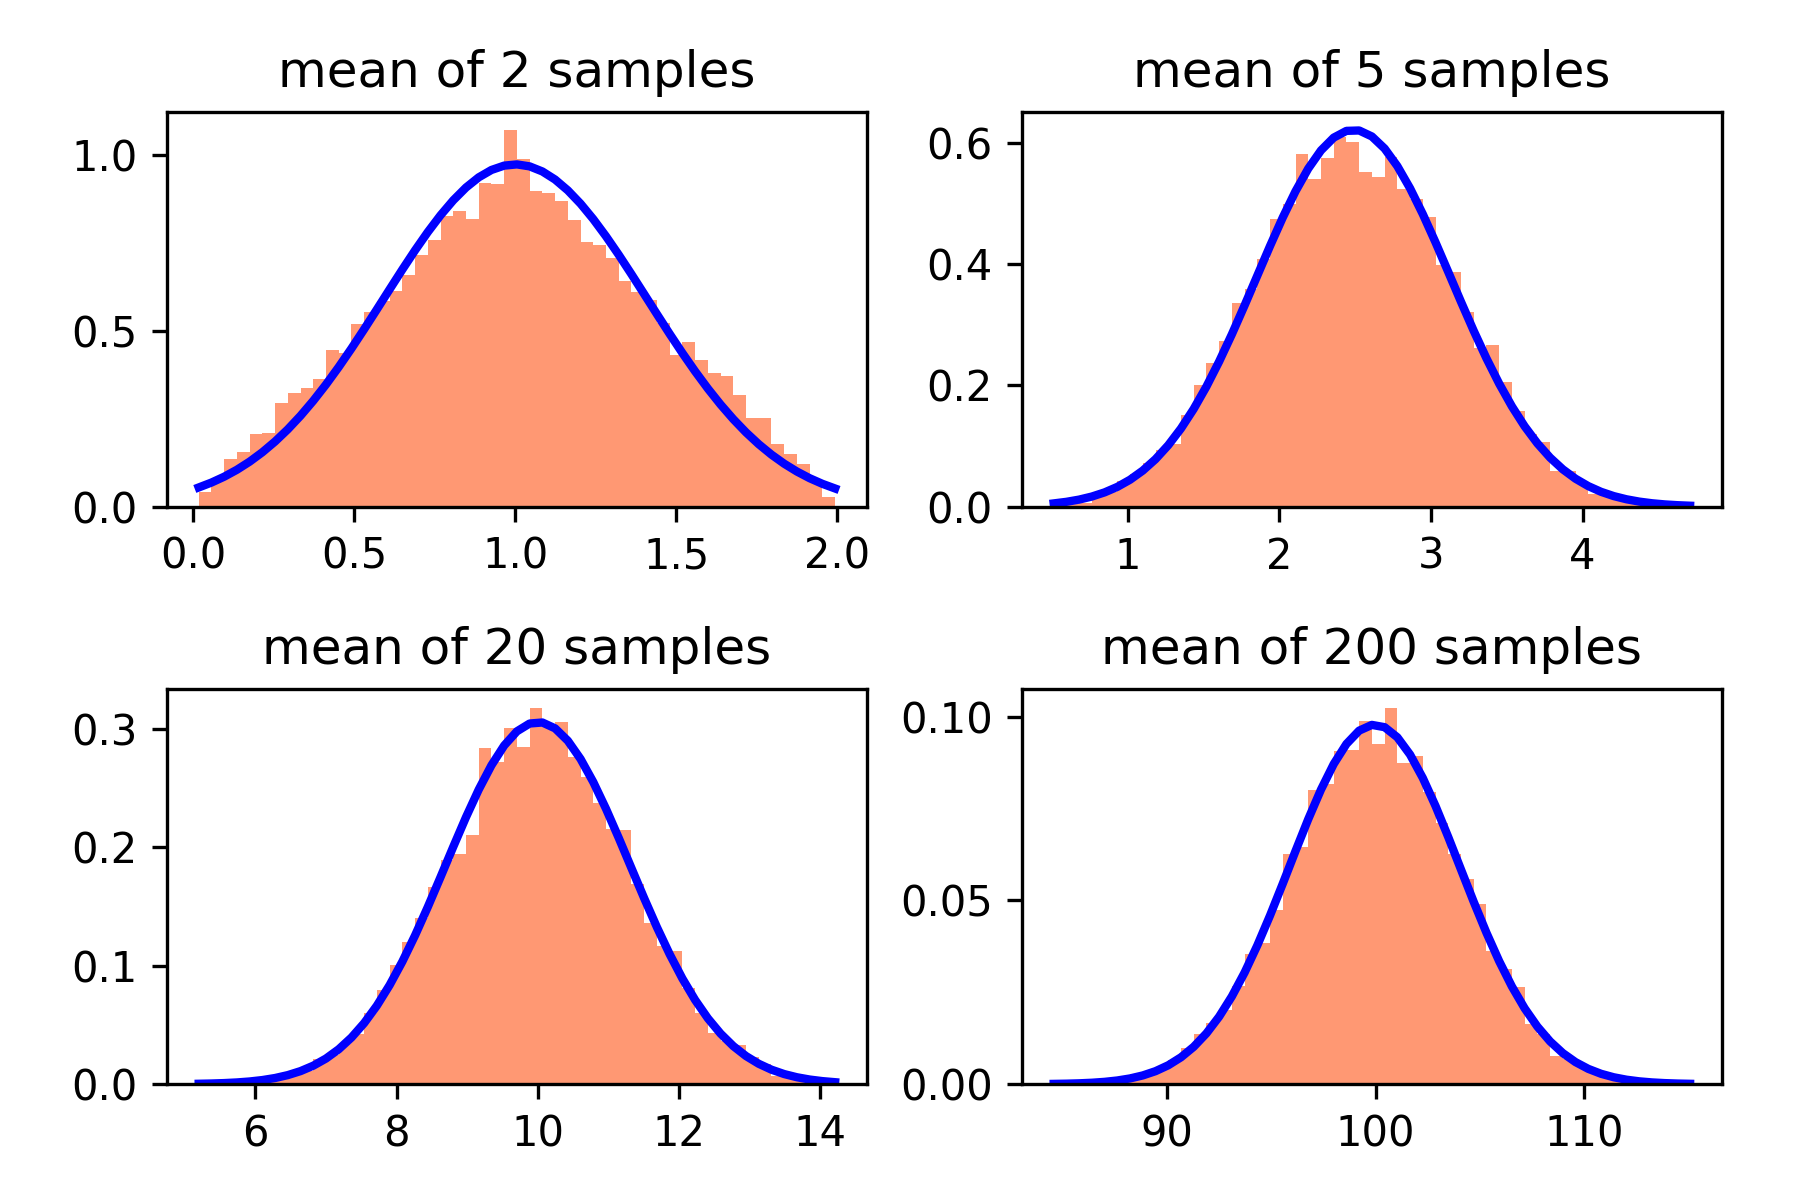
\includegraphics[width=\textwidth]{1a}
	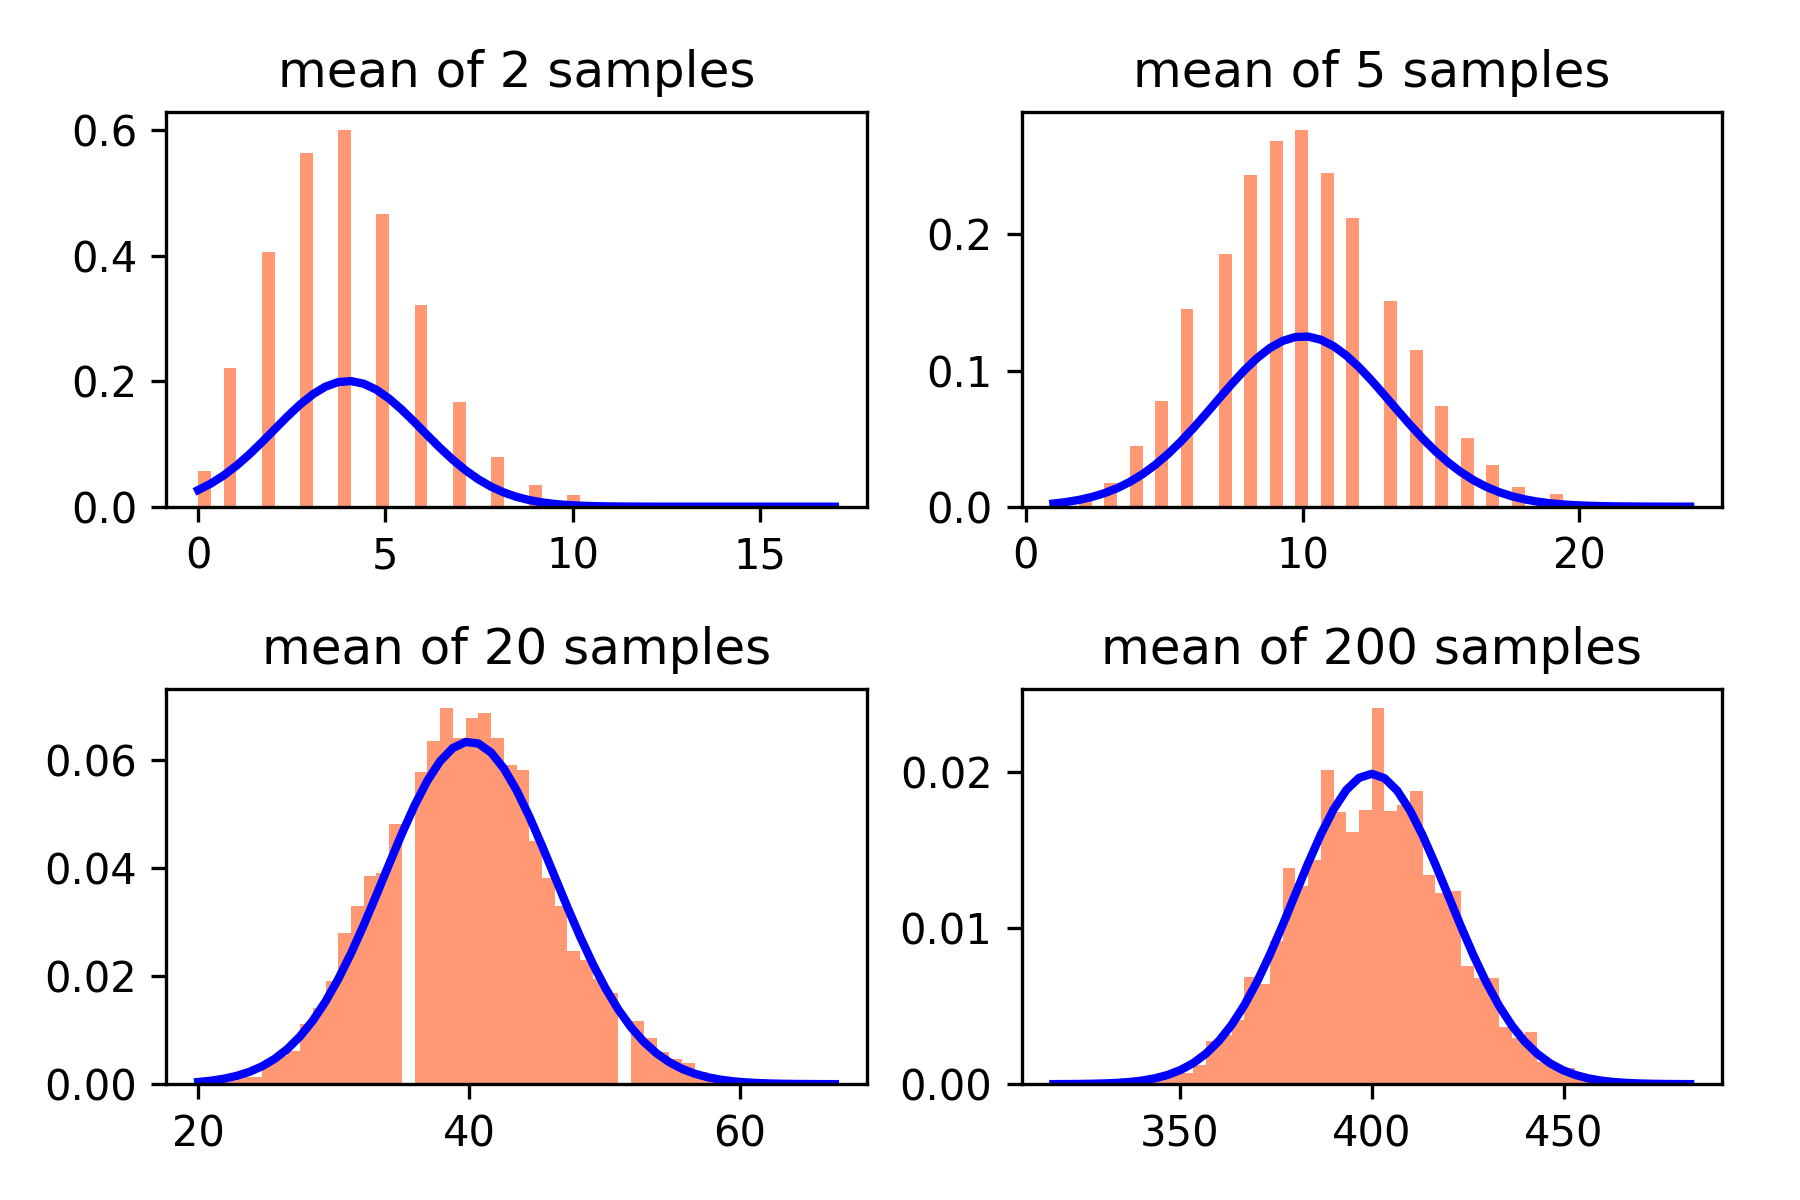
\includegraphics[width=\textwidth]{1b}

	\begin{problem}
		Go to \url{exoplanets.org} and obtain the distribution of stellar [Fe/H]. For this, go to the ``Plots'' tab and click on the “Histogram Plot” and ``Advance'' tabs (on the right). Using the ``Data'' pull- down menu (which is below the ``Simple'' and ``Advance'' tabs) choose FE (almost at the end of the menu, under “Stellar Properties”). Choose the min and max of the [Fe/H] values to be $-0.5$ and $0.5$, respectively, and a binwidth of $0.04$ (this should give you 25 bins), using all stars with exoplanets and measured values of [Fe/H].

		Use this distribution as the parent pdf. Write a code to obtain $10^5$ randomly distributed points from this parent distribution. Plot a histogram of the value of the points obtained from your code and compare it with a plot of the parent distribution. Are the two distributions similar? How would you test if these two distributions come from the same parent distribution?
	\end{problem}
	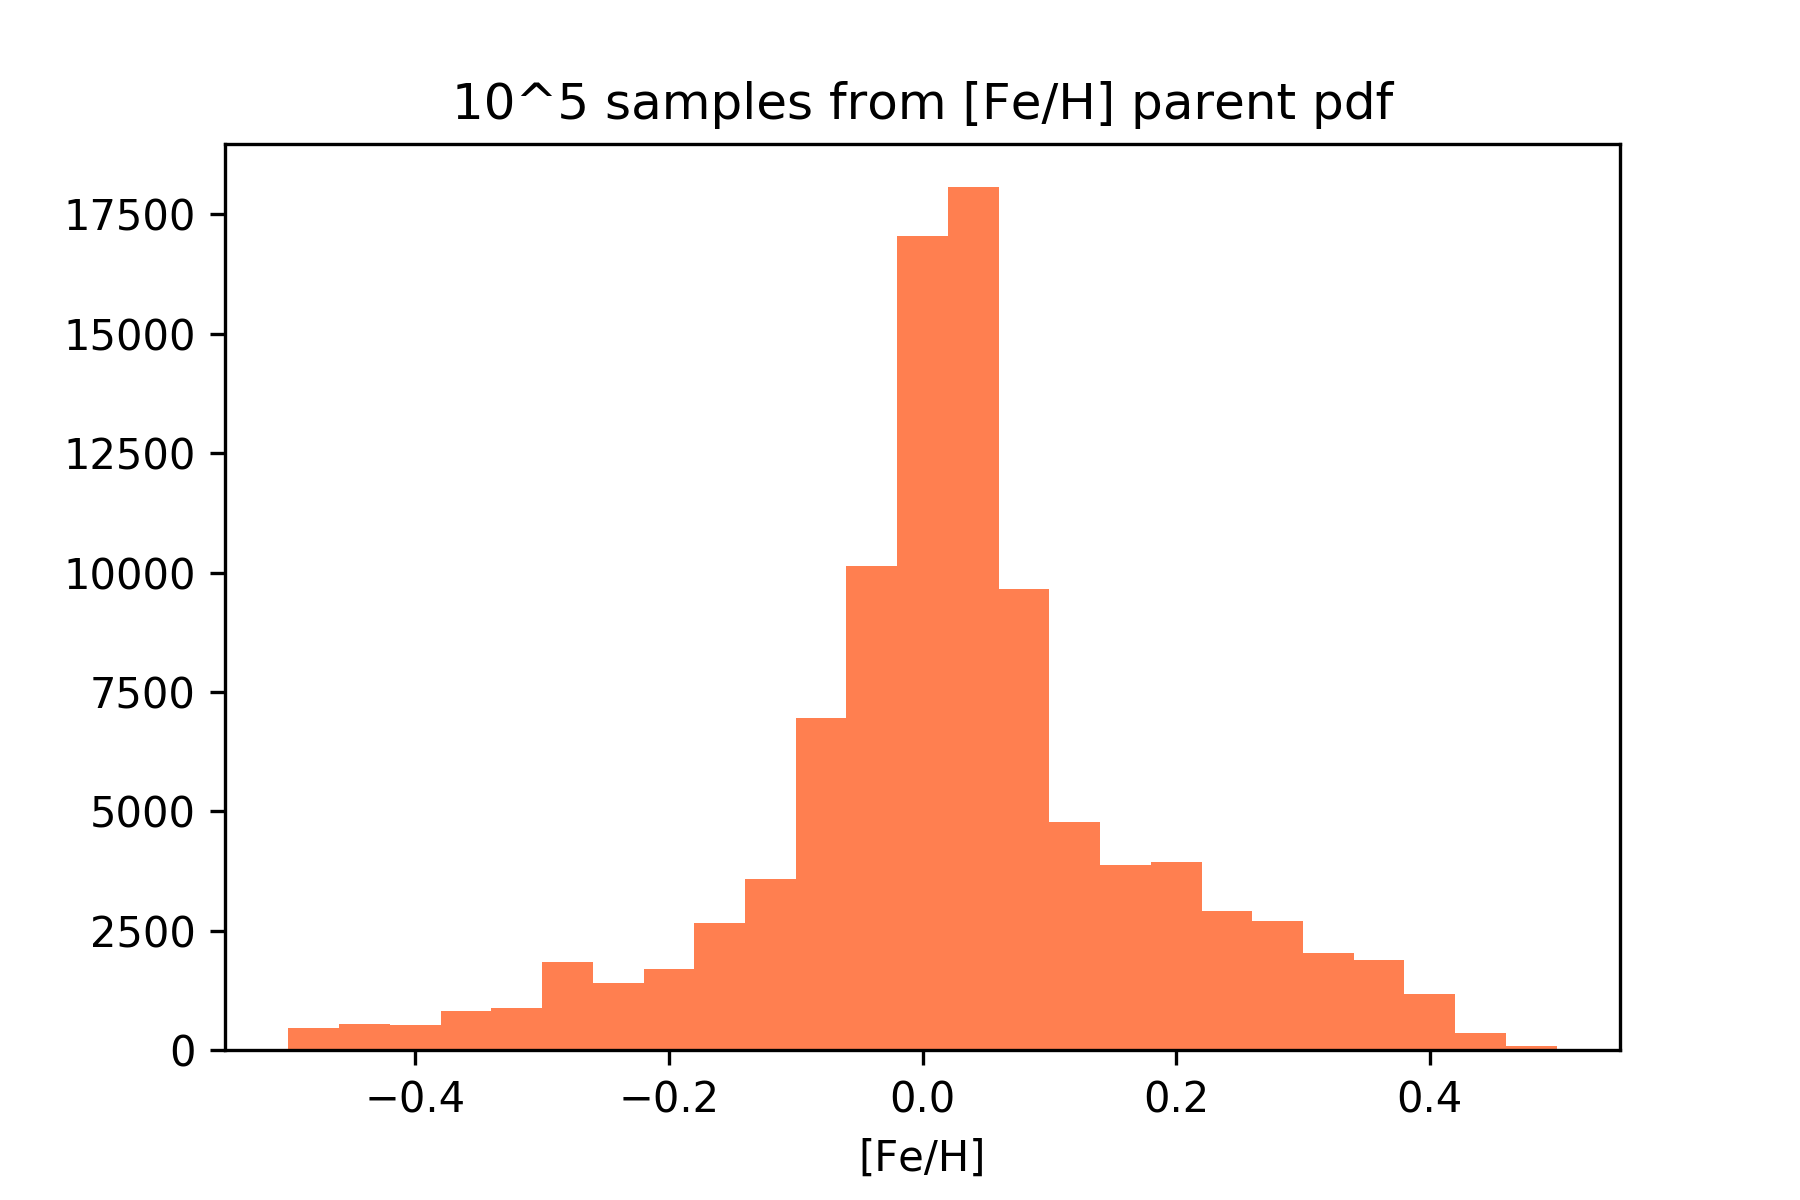
\includegraphics[width=\textwidth]{2}
	\begin{proof}[Solution]
		The plots are indeed quite similar.
		In order to get a quantifiable metric on how distinct the two distributions are (and thereby determine if they have the same parent distribution), we can preform a non-parametric test like a Komologorov-Smirnov test.
	\end{proof}

	\begin{problem}
		Suppose you have bivariate data $(x_1,y_1),\dots,(x_n,y_n)$.
		A common model is that there is a linear relationship between $x$ and $y$, so in principle the data should lie exactly along a line.
		However since data have random noise and our model is probably not exact this will not be the case.
		What we can do is look for the line that best fits the data.
		To do this we will use a simple linear regression model.
		For bivariate data the simple linear regression model assumes that the $x_i$ are not random but that for some values of the parameters $a$ and $b$ the value $y_i$ is drawn from the random variable $Y_i \sim ax_i +b+\varepsilon_i$, where $\varepsilon_i$ is a normal random variable with mean $\mu = 0$ and variance $\sigma^2$.
		We assume all of the random variables $\varepsilon_i$ are independent.
		\begin{parts}
			\part[part:3:a] The distribution of $Y_i$ depends on $a$, $b$, $\sigma$ and $x_i$.
			Of these only $a$ and $b$ are not known.
			Give the formula for the likelihood function $f\qty(y_i \mid a, b, x_i, \sigma)$ corresponding to one random value $y_i$. %

			\part[part:3:b] 
				\begin{enumerate}[label=\textup{(\roman*)}]
					\item\label{part:3:b:i} Suppose we have data (1, 8), (3, 2), (5, 1).
					Based on our model write down the likelihood and log likelihood as functions of $a$, $b$, and $\sigma$.%

					\item\label{part:3:b:ii} For general data $(x_1,y_1), \dots, (x_n,y_n)$ give the likelihood and log likelihood functions (again as functions of $a$, $b$, and $\sigma$).
				\end{enumerate}%

			\part[part:3:c] Assume $\sigma$ is a constant, known value. 
			For the data in part b(i) find the maximum likelihood estimates for $a$ and $b$.
			Give confidence intervals for your estimates of $a$ and $b$.%

			\part[part:3:d] Use python to plot the data and the regression line you found in 1c.
		\end{parts}
	\end{problem}
	\begin{proof}[Solution to~\ref{part:3:a}]
		If $y_i$ is related to $x_i$ through
		\[ y_i \sim ax_i + b - \varepsilon_i, \]
		where $\varepsilon_i \sim \mathcal{N}(\mu, \sigma^2)$, let $\vb*{\theta}$ be a tuple representing our parameters $\vb*{\theta} = (x_i ;a, b, \sigma)$.
		We know that $f(y_i \mid \vb*{\theta})$ represents the probably density function for $y_i$ given the parameters of $\vb*{\theta}$.
		In general, we know that the likelihood function for a set of $n$ observations $y_i$ is given by
		\begin{equation} 
			\mathcal{L}(\vb*{\theta} \mid \vb{y}) = \prod_{i = 1}^n f(y_i \mid \vb*{\theta}),\label{eqn:1:lik}
		\end{equation}
		and so for a single observation $y_i$, the likelihood function for one random value is simply
		\[ \final{\mathcal{L}(\vb*{\theta} \mid y_i) = f(y_i \mid \vb*{\theta}) = \frac{1}{\sqrt{2\pi\sigma^2}}\e^{(y_i-[b+ax_i])^2/(2\sigma^2)},}\qedhere \]
		since if $\varepsilon_i$ is normally distributed then $y_i \sim \mathcal{N}(ax_i + b, \sigma^2)$.
	\end{proof}
	\begin{proof}[Solution to~\ref{part:3:b}\ref{part:3:b:i}]
		By equation~\eqref{eqn:1:lik}, we know that
		\[
			\mathcal{L}(\vb*{\theta} \mid \vb{y}) = \prod_{i=1}^n f(y_i \mid \vb*{\theta}).
		\]
		Since our data is normally distributed, we know by part~\ref{part:3:a} the form that the likelihood function will take.
		Then for the particular set of obsernations, $\{(1,8),(3,2),(5,1)\}$ the total likelihood function is then
		\begin{align*}
			\mathcal{L} &= \qty[\frac{1}{\sqrt{2\pi\sigma^2}}]^3\cdot\exp\qty(\frac{(8-[b+a])^2 + (2 - [b+3a])^2 + (1 - [b+5a])^2}{2\sigma^2}) \\
			&= \final{\qty[\frac{1}{\sqrt{2\pi\sigma^2}}]^3\cdot\exp\qty(\frac{35 a^2 + 18 a b - 38 a + 3 b^2 - 22 b + 69}{2\sigma^2}).}
		\end{align*}
		The log likelihood of this is then
		\begin{align*}
			\ln\mathcal{L} &= -\frac{n}{2}\ln(2\pi) - n\ln(\sigma) - \frac{1}{2\sigma^2}\qty[\qty(8-[b+1])^2 + \qty(2-[b+3a])^2 + \qty(1 - [b+5a])^2]. \\
			&= \final{-\frac{n}{2}\ln(2\pi) - n\ln(\sigma) - \frac{1}{2\sigma^2}\qty[35 a^2 + 18 a b - 38 a + 3 b^2 - 22 b + 69].}\qedhere
		\end{align*}
	\end{proof}
	\begin{proof}[Solution to~\ref{part:3:b:ii}]
		Let $\vb{y} = (y_1,y_2,\dots,y_n)$ be the set of $n$ observations based on the parameters $\vb*{\theta}$.
		For a set of $n$ iid observations, we know that the likelihood function for those observations is given by
		\[ \mathcal{L}\qty(\vb*{\theta}) = \prod_{i = 1}^n f(y_i \mid \vb*{\theta}) = \final{\prod_{i = 1}^n \frac{1}{\sqrt{2\pi\sigma^2}}\e^{(y_i-[b+ax_i])^2/(2\sigma^2)}.}\]
		The log likelihood transforms this into
		\begin{align*}
			\ln\mathcal{L}(\vb*{\theta}) &= \sum_{i = 1}^n \ln \frac{1}{\sqrt{2\pi\sigma^2}}\e^{(y_i-[b+ax_i])^2/(2\sigma^2)} \\
			& = \final{-\frac{n}{2}\ln(2\pi) - n\ln(\sigma) - \frac{1}{2\sigma^2}\sum_{i=1}^n\qty(y_i - [b + ax_i])^2.}\qedhere
		\end{align*}
	\end{proof}
	\begin{proof}[Solution to~\ref{part:3:c}]
		In order to maximize our likelihood estimates, we need to differentiate our likelihood function (or log likelihood) with respect to the subset of parameters $\vb*{\theta^*} = (a,b)$ we wish to account for.
		So
		\begin{align*}
			\pdv{\ln\mathcal{L}(\vb*{\theta} \mid \vb{y})}{\vb*{\theta^*}} = 0 \implies \pdv{\vb*{\theta^*}}\qty[-\frac{1}{\sigma^2}\sum_{i=1}^n \qty(y_i - [b + ax_i])^2] = 0,
		\end{align*}
		Since all other terms are constant in $a,b$.
		Evaluating these derivatives separately, we see that
		\begin{align*}
			\pdv{\ln\mathcal{L}(\vb*{\theta} \mid \vb{y})}{a} &= \frac{1}{\sigma^2}\sum_{i=1}^n x_i\cdot(y_i - [b + ax_i]), \\
			\pdv{\ln\mathcal{L}(\vb*{\theta} \mid \vb{y})}{b} &= \frac{1}{\sigma^2}\sum_{i=1}^n (y_i-[b+ax_i]).
		\end{align*}
		When this system is minimized, we get that
		\begin{align*}
			\sum_i y_i - b - ax_i = 0, \quad\text{and}\quad\sum_i y_ix_i - bx_i -ax_i^2 = 0,
		\end{align*}
		which we can simplify using the arithmetic means of $x_i$ and $y_i$ to 
		\[ \bar{y}-b-a\bar{x} = 0,\quad\text{and}\quad \bar{y}\bar{x}-b\bar{x}-a\bar{x}^2 = 0. \]
		This tells us that the maximum likelihood estimates for $a$ and $b$ are
		\[ \hat{b} = \bar{y} - \hat{a}\bar{x},\quad\text{and}\quad \hat{a} = \frac{\text{Cov}(x,y)}{\text{Var}(x)} = \frac{\sum (x_i-\bar{x})(y_i-\bar{y})}{\sum(x_i-\bar{x})^2}. \]
		For the data given in part~\ref{part:3:b:i}, we see that
		\[ \text{Cov}(x,y) \approx -4.67,\quad\text{Var}(x) \approx 14.33 \implies \final{\hat{a} = -3.07,\quad \hat{b} = 12.88.}\]
		Since our data was initially drawn from a distribution approximating $\mathcal{N}(ax_i+b,\sigma^2)$, and we have drawn 3 samples, then the standard error for our estimates of $a$ and $b$ should be 
		\[ \text{error} = \pm N\cdot\frac{\sigma}{\sqrt{3}}, \]
		where $N$ is 
	\end{proof}
	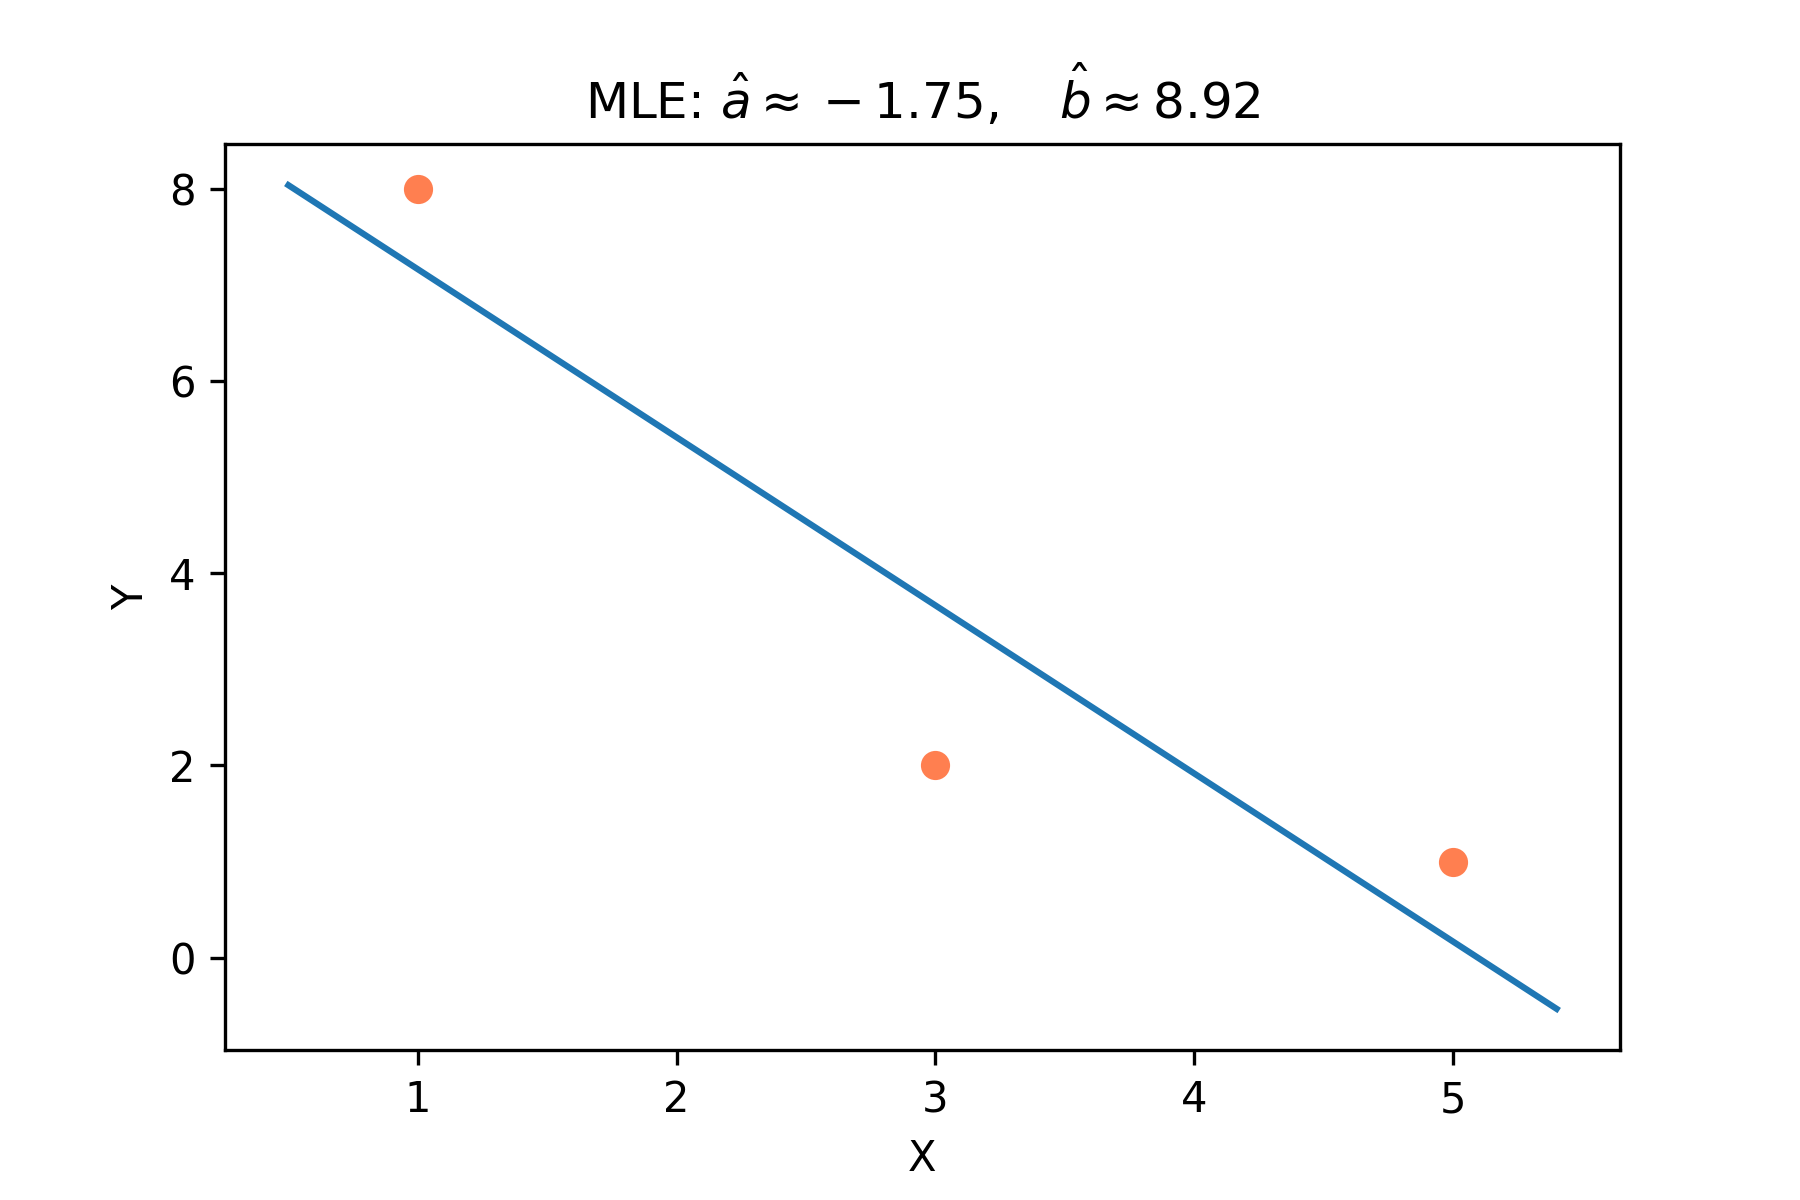
\includegraphics[width=\textwidth]{3d}
	
	\begin{problem}
		Estimating parameters of a uniform distribution.
		\begin{parts}
			\part[part:4:a] Suppose we have data $1.2, 2.1, 1.3, 10.5, 5$ which we know is drawn independently from a uniform distribution $\sim \mathcal{U}(a,b)$.
			Give the maximum likelihood estimate for the parameters $a$ and $b$.
			Recall that the pdf for $\mathcal{N}(a,b)$ is 
			\[ 
				f(x \mid a,b) = \begin{cases}
					\frac{1}{b-a}, & a \leq x \leq b \\
					0, & \text{otherwise}.
				\end{cases}
			\]
			\part[part:4:b] Suppose we have data $x_1,x_2,\dots,x_n$ which we know is drawn independently from a uniform distribution $\sim \mathcal{U}(a,b)$.
			Give the maximum likelihood estimate for the parameters $a$ and $b$ in mathematical form.
		\end{parts}
	\end{problem}
	\begin{proof}[Solution to~\ref{part:4:a}]
		We know that the interval $[a,b]$ must contain all our observations, or else they cannot have been drawn from the uniform distribution.
		Notice that $f \propto 1/(b-a)$, so to maximize the probability (and hence the likelihood), we must minimize $b-a$.
		This entails making our bounds as close as possible to the extrema of our data.
		If we set the upper bound $b$ to be the largest point in our dataset, and $a$ to be the smallest, then $b-a$ is as small as it can be.
		Then for the example data, our estimators for $a$ and $b$ should be
		\[ \final{\hat{a} = 1.2,\qquad\hat{b}=10.5.}\qedhere \]
	\end{proof}
	\begin{proof}[Solution to~\ref{part:4:b}]
		As we've established, if $f(x \mid \vb*{\theta})$ is the probably distribution for a single independent event, then for $n$ samples $\vb{x}$ we see that for a fixed $a,b$ our probability is
		\[  
			f(\vb{x} \mid \vb*{\theta}) = \begin{cases}
				\qty(\frac{1}{b-a})^n, & a \leq x \leq b \\
				0, & \text{otherwise}.
			\end{cases}	
		\]
		This is maximized when $b-a$ is as small as possible, under the condition that $x_i \in [a,b]$ for all $i$.
		Then our system is maximized when
		\[ \final{\hat{a} = \text{min}(x_1,\dots,x_n),\qquad\hat{b} = \text{max}(x_1,\dots,x_n).}\qedhere \]
	\end{proof}
\end{document}